\documentclass[10pt, titlepage]{report}

\usepackage[utf8]{inputenc}
\usepackage[T1]{fontenc}
\usepackage[francais]{babel}

%Caractères spéciaux

\usepackage{lmodern}
\usepackage{amsmath}
\usepackage{amssymb}
\usepackage{mathrsfs}

\usepackage{eurosym} %insertion signe euro
\usepackage{graphicx} %insertion d'images
\usepackage{fancyhdr} %en-tete et pied de page

\title{\bsc{Rapport de la première soutenance}\\Projet flight arena}
\author{mr cube :\\
Vincent \bsc{Rospini-Clerici},\\
Guillaume \bsc{Rebut}\\
%Nikolas \bsc{Miletic}\\
chef de projet : Arthur \bsc{Remaud}}
\date{12 mars 2015}

\pagestyle{fancy}
\fancyhead{}
\fancyfoot{}
\lhead{Rapport de la première soutenance}
\rhead{Projet Flight Arena}
\lfoot{mr cube}

\begin{document}

\maketitle
\renewcommand{\contentsname}{Sommaire}
\renewcommand{\chaptername}{Partie}

\tableofcontents

\chapter{Modification du cahier des charges}
Suite au départ de Nikolas Miletic en S1\#, nous avons dû modifier le cahier des charges pour réajuster le budget et répartir à nouveau les tâches entre les trois membres restant.\\

Au niveau du budget, en terme de matériels, nous sommes passé de 3800 \euro à 2100 \euro, car l'ordinateur de Nikolas coûte 1700 \euro. Le budget total est donc passé de 5397,29 \euro à 3697,29 \euro. Le budget pour les logiciels n'a pas évolué.\\

Pour la répartition du travail, le script dont était chargé Nikolas a été confié à Arthur, Guillaume s'est chargé entièrement du gameplay. Nous avons malgré tout pris du retard pour ce qui est du son et de la gestion des données.

Le son a été pris sur internet ou sur d'autres logiciels existant déjà, alors que nous avions prévu de le faire nous-même. A cause de la baisse de main-d'œuvre, nous n'avons plus le temps nécessaire de le faire, et nous préférons accorder plus de temps au jeu lui-même. La gestion des données dont devaient se charger Arthur et Nikolas n'a quasiment pas été commencée, car nous avons voulu privilégier le script principal du jeu.\\

Pour les soutenances à venir, nous avons donc renoncé à faire le son, mais nous devrons nous rattraper pour les données afin d'avoir au moins des sauvegardes. Nikolas devait aussi s'occuper de l'I.A et du site web. C'est donc Guillaume et Arthur qui vont faire l'I.A, et le site web sera construit par toute l'équipe.\\

\chapter{Retard/Avance par rapport au cahier des charges}
Les retards que nous avons par rapport aux prévisions du cahier des charges sont principalement causées par le départ d'un membre. Si nous regardons ce que nous nous avions fixé par personne, nous sommes dans les temps. 

\section{Retard}

\paragraph{Son :}
Nous n'avons que très peu de fond sonore pour l'instant. Nous avons actuellement pris la musique du menu principal du jeu sur internet au lieu de la faire par nos propres moyens : il s'agit de \textit{Captain America March}. Nous ne ferons probablement pas la musique du jeu, car cela nous prendrait trop de temps.

 Par contre, un ami de Vincent qui est en étude de musicologie a accepté de faire des musiques pour le jeu sur un thème symphonique, comme les musiques de Star Wars, et électroniques.\\

 Pour le son des tirs, nous avons pris un bruitage du jeu Pinball sur Windows XP qui ressemble à un son de laser. Nous rajouterons des bruitages lors du crash du vaisseau quand celui-ci sera implémenté et le bruit des réacteurs du vaisseau.

\paragraph{Gestion des données :}
Il n'y pas pour l'instant de gestion des données, ou du moins pas visible pour le joueur. En effet, il n'y a pas de sauvegardes dans le jeu ou de munitions, et la vie du joueur ne s'affiche pas à l'écran. Le menu option ne comporte pour l'instant que la modification du volume du jeu, qui est cependant conservée même après avoir fermé le jeu.

\section{Avance}

\paragraph{Gameplay :}
Le gameplay est plus avancé que ce que nous espérions. Nous avons déjà un vaisseau opérationnel avec des contrôles qui fonctionnent assez bien. Nous avons modélisé plusieurs bâtiments qui offrent un environnement agréable et permet déjà de s'amuser à piloter dans le décor sans trop de difficultés. On peut aussi tirer dans le jeu avec la touche \textit{espace}. Le jeu est donc déjà jouable, même s'il n'y a pas d'ennemis, car la prise en main du vaisseau est déjà un défi en soi.

On a donc toutes les bases d'un gameplay de jeu de vaisseau : un vaisseau que l'on peut piloter, une carte de jeu avec des bâtiments qui nous obligent à zigzaguer pour les éviter, et les tirs pour tuer le joueur adverse. Il ne manque plus que la mort et les ennemis pour avoir l'intégral du gameplay de notre jeu final, ce qui sera fait pour les soutenances à venir.

\paragraph{Script :}
Nous sommes en avance sur le script de base du jeu. Unity contient énormément de fonctions prédéfinies qui aident grandement à générer rapidement du code en C\#. Les contrôles se font simplement par des fonctions qui déplacent ou tourne le vaisseau de lui-même, et les balles tirés sont instanciées simplement en définissant le point de départ de l'apparition puis en les déplaçant droit devant elles.

 Nous n'avons pas eu besoin de faire de script pour la caméra : en la reliant au vaisseau dans Unity, elle suit le automatiquement en fonction de ses déplacement. Nous avons fait de même pour le point de départ des balles.

 Nous avons aussi bien avancé les menus, que ce soit le menu principal du jeu avec les options, ou le menu de pause dans le niveau que nous avons créé.

\paragraph{Moteur physique :}
La physique du jeu est quasiment terminée. En effet Unity permet de faire la physique du jeu et les collisions très facilement, en appliquant des collider directement sur les objets qui en prennent la forme. Les vaisseaux ont donc déjà leurs propriétés physique et entrent en collision avec les bâtiments.

 Les bords du niveau sont aussi faits, si bien que si le joueur tente de trop s'éloigner du niveau, il rencontre un mur invisible qui l'empêche d'avancer plus loin. Il ne peut donc pas faire planter le jeu en allant trop loin. 

Le nombre de balles est aussi gérer, car elles s'autodétruisent au bout de quelques secondes. Il n'y a donc pas de saturation de mémoire parce qu'il y aurait trop d'objets.

\chapter{Travail par membre}
Nous allons vous décrire ce que chaque membre de l'équipe mr cube a fait pendant cette première période, avec leurs difficultés rencontrées et les techniques utilisées.

\section{Guillaume Rebut}

Notre jeu est un shooter multijoueur où le joueur est aux commandes d'un vaisseau et combat d'autres vaisseaux sur des petites arènes. Un jeu de bonne qualité se doit d'être facile à prendre en main mais difficile à maitriser. Pour répondre à cette exigence, nous avons décidé de créer les mouvements des vaisseaux en se basant sur les avions de chasses.\\

 Les vaisseaux ont trois types de mouvements : le roulis, rotation du vaisseau selon l'axe longitudinale, le tangage , rotation du vaisseau sur son axe transversal, et le lacet, rotation du vaisseau selon l'axe vertical. Les vitesses de rotations s'inspirent aussi des valeurs des avions: le tangage est plus rapide que le roulis qui est bien plus rapide que le lacet (les valeurs finales ne sont pas encore déterminées).

 Nous avons aussi choisi de prendre ces valeurs pour des raisons de gameplay. En effet, il est plus facile de tourner avec le lacet plutôt que d'utiliser la combinaison tangage plus roulis. Il est donc logique de rendre cette dernière manœuvre plus rapide en exécution pour récompenser les joueurs les plus talentueux.

 Nous avons aussi placé la caméra de manière à inciter le joueur à utiliser cette dernière manœuvre : le vaisseaux n'est pas représenté au milieu de l'écran mais en bas pour donner plus de visibilité. Toujours dans une optique de réalisme et de difficulté, le vaisseau a de l'inertie et ne peut pas reculer.\\

Le vaisseau est entièrement contrôlable au clavier. Les touches directionnelles représentent un joystick d'avion et permettent le tangage (flèche du haut pour piquer et flèche du bas pour "monter") et le roulis (flèche gauche pour une rotation anti-horaire et flèche droite pour une rotation horaire). La touche W permet l'accélération et les touches A et D permettent de tourner respectivement à gauche et à droite grâce au lacet.\\

Les décors occupent une place importante dans le gameplay. Notre niveau contient des buildings de tailles importantes par rapport au vaisseau qui devra les éviter, au risque d'exploser, ce qui augmente la difficulté des manœuvres.

Les buildings présentent aussi un aspect défensif important: lorsqu'un vaisseau chasse un autre vaisseau, ce dernier peut s'échapper en se faufilant entre les buildings, en manœuvrant dans le parking ou en se cachant. 

\section{Vincent Rospini-Clerici}

\subsection{Modélisation du vaisseau}

Après le visionnage de différents tutoriels Blender sur la modélisation d'objets 3D, Vincent a commencé le premier vaisseau qui sera utilisé par le joueur dans le jeu. C'était la première fois qu'il utilisait le logiciel Blender. Il s'est servi principalement de la fonction extrude en partant d'un simple cube pour parvenir à modéliser ce qu'il souhaitait. Cette fonction permet en effet d'avoir un vaisseau en un seul objet plus aisément qu'en utilisant l'ajout de \textit{mesh}. Par exemple, en coupant les solides en différentes parties grâce à l'outil \textit{knife}, cela a permis d'extraire la forme basique des ailes à partir du corps principal du vaisseau.\\

Il a aussi utilisé le modifier \textit{mirror} qui est très important. Il permet de créer une image reproduite de l’objet créé par Rapport à un axe. Ce qui permet au vaisseau d'être parfaitement symétrique.\\

Vincent a également utilisé le modifier \textit{subdivision surface} pour créer des surfaces de subdivision, c’est-à-dire découper les faces de l’objet en plusieurs afin de le lisser. Ce modifier appliqué sur l’ensemble du vaisseau lui donne cet aspect rond et c’était exactement ce qu’il fallait pour coller aux graphismes du jeu.
Une fois la modélisation terminée, il a fallu également texturer toutes les faces du vaisseau afin d'avoir un beau rendu dans le jeu.\\

Pour se faire, il a fallu se servir de l'outil \textit{UV Mapping} qu'offre Blender. Il s'agit de sélectionner toutes les arrêtes du vaisseau et de les déplier sur un plan en deux dimensions. Le logiciel Photoshop permet ensuite de remplir les différentes faces avec les couleurs et textures voulues. Le vaisseau a pour l'instant été texturé entièrement en rouge et noir avec des dégradés de couleur. Mais, des différentes versions de textures de ce vaisseau seront peut-être ajoutées pour permettre au joueur de choisir la couleur de son vaisseau.\\

Les vaisseaux suivants seront sûrement réalisés avec ces mêmes procédés.

\begin{figure}
\center
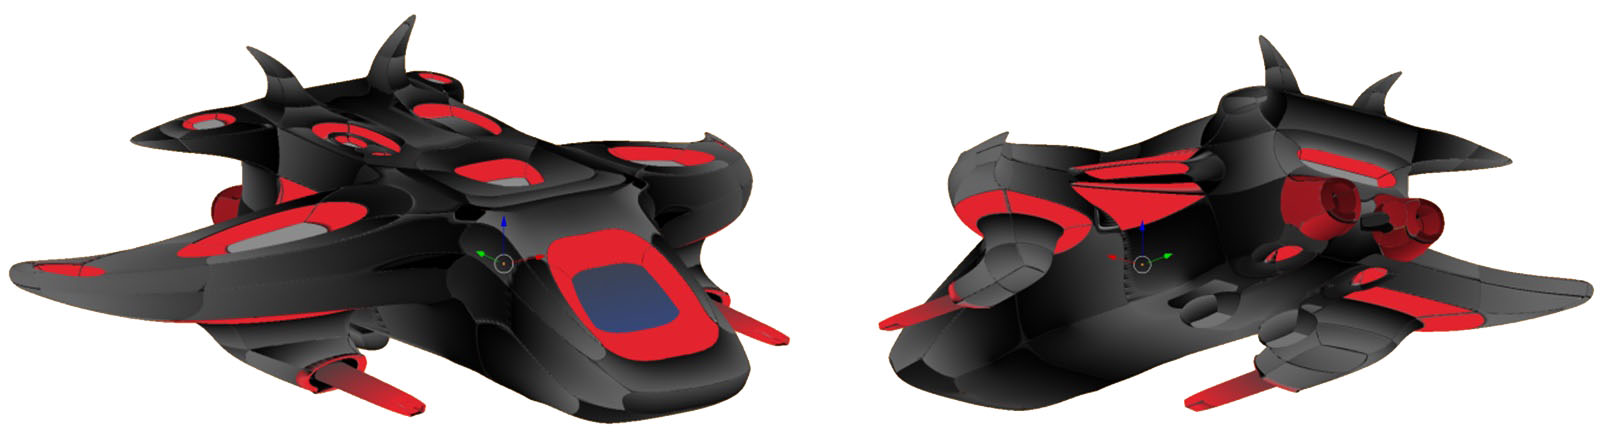
\includegraphics[height=4.5cm, width=15cm]{vaisseau_vincent.jpg}
\caption{Le vaisseau principal fait par Vincent}
\end{figure}

\subsection{Modélisation des bâtiments}

Vincent a créé sept bâtiments différents et entièrement texturés pour les besoins de la première carte. Ils ont tous des formes et des hauteurs différentes car ils ont permis de tester comment Unity gérait les collisions entre le vaisseau et les objets.\\

Ces bâtiments ont été créés sur Blender et texturés sur Photoshop de la même façon que le vaisseau.

\begin{figure}
\center
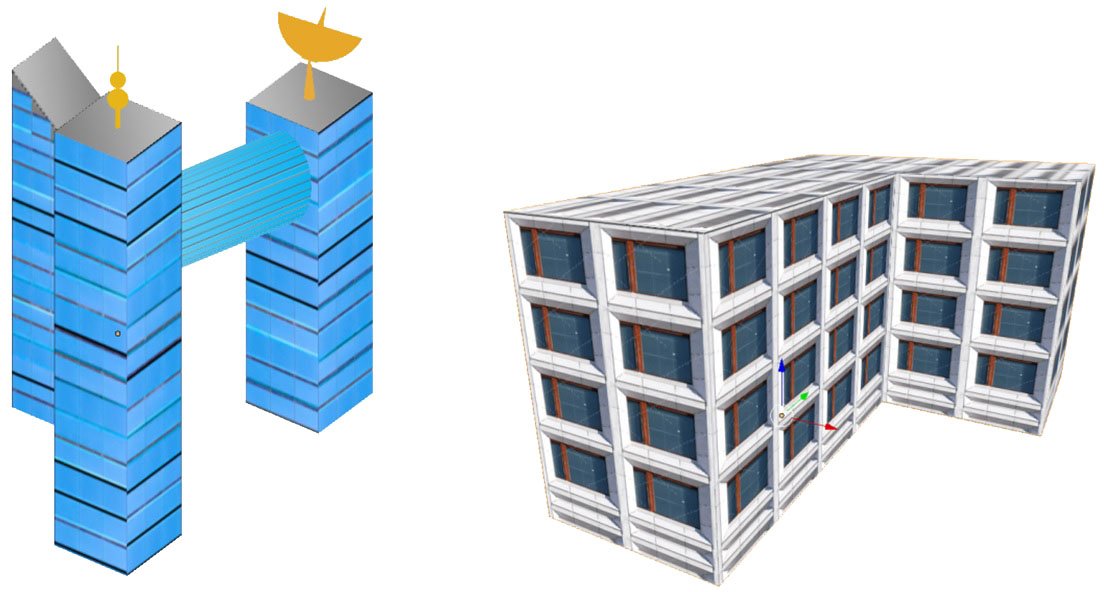
\includegraphics[height=6cm, width=11cm]{batiments_vincent.jpg}
\caption{Deux bâtiments faits par Vincent}
\end{figure}

\subsection{Différents problèmes rencontrés}

De nombreux problèmes ont été rencontrés lors de la création de textures pour le vaisseau.\\

Au moment de passer l’\textit{Uv Mapping} de Blender pour le vaisseau, le vaisseau texture, Blender affichait le vaisseau avec des problèmes de symétrie. C’était en réalité du au modifier \textit{bevel} qui était censé entre autre biseauter les faces du vaisseau. En l’enlevant, Vincent a réalisé que le vaisseau était bien mieux avec le modifier  \textit{Subdivision Surface} qu’avec le modifier \textit{Bevel} et que les problèmes de symétrie disparaissaient.\\

Un autre problème est survenu lors du dépliage des faces du vaisseau par l’\textit{Uv mapping}.

Le vaisseau ayant plus de trois cent faces, Vincent a décidé de découper l’\textit{Uv mapping} par patrons, mais cette tâche s’est révélée très complexe et lorsque Vincent a déplié le patron du vaisseau, les faces étaient méconnaissables et toutes empilées les unes sur les autres. Il a donc fallu qu’il opte pour une autre méthode. Il a sélectionné toutes les faces du vaisseau, puis il les a dépliées toutes indépendamment. Finalement il a fallu repérer toutes les faces et les regrouper par endroit du vaisseau (ailes, avant, etc...)

\subsection{Ce que Vincent doit faire pour la seconde soutenance}
Il faut modéliser et texturer au moins un autre vaisseau sur Blender pour créer du contenu dans le jeu. Un autre vaisseau a d’ailleurs été ébauché.
Modéliser la destruction du vaisseau lors d'un crash et l'implémenter au code est indispensable pour la prochaine soutenance. Nous pensons d’ailleurs que la fonction \textit{explode} pourra nous être très utile pour que le vaisseau éclate en plusieurs morceaux.\\

Il faudra évidemment implémenter les flammes des réacteurs des vaisseaux afin que le joueur n’ai pas l’impression que le vaisseau avance tout seul sans raison..
Les premiers sons qui sont actuellement dans le jeu sont basiques. Il s’agirait d’en rajouter d’autres avant la seconde soutenance.\\

Enfin, il faudra commencer le site internet et en faire la majeure partie. Il sera a priori créé grâce au logiciel Adobe Dreamweaver.


\section{Arthur Remaud}
Pendant cette première période, Arthur a fait tous les scripts en C\# du jeu et quelques modélisations 3D rapides avec blender.

\subsection{Scripts}

Tous les scripts en C\# du jeu ont été fait par Arthur grâce à des tutoriels sur internet. La fonction $Input.GetKey()$ de Unity permet de lire tout ce que l'utilisateur entre sur le clavier. Il a donc enregistré les différentes saisies possibles du joueur, qui provoquent sur le vaisseau des translations avec la fonction $transform.Translate()$ lorsque le joueur veut avancer ou des rotations avec la fonction $transform.Rotate()$ lorsque le joueur veut tourner. Chacun peut donc aisément piloter le vaisseau pour éviter les obstacles. L'inertie du vaisseau est géré par une variable de déplacement qui augmente à force d'appuyer sur la touche d'accélération, et diminue dans le cas contraire.\\

Il a aussi mis une touche pour tirer avec le vaisseau. Dans ce cas Unity crée une instance de la balle (fonction $Instantiate()$) qui part droit devant. Elle disparait automatiquement au bout de quelques secondes grâce à la fonction $DestroyObject()$, le temps d'au moins traverser le terrain, pour éviter d'avoir trop d'objets à la fois qui partent vers l'infini, ce qui provoquerait un ralentissement du jeu.

La balle contient aussi un \textit{trigger} qui s'active lors d'une collision. Si le joueur entre en collision avec une balle, alors celle-ci est détruite et le joueur perd de la vie.

La principale difficulté rencontrée fut la gestion de l'inertie lorsque l'objet est touché par le décor. En effet, il peut rapidement partir en vrille et n'est plus maniable. Après des recherches sur internet, il est apparu que le problème venait du \textit{rigidbody} et c'est la vélocité de celui-ci qu'il faut remettre à zéro à chaque fois.\\ \\

 Il a aussi fait les menus, en utilisant les propriétés GUI (Graphical User Interface) de Unity. Il a pris une police avec un effet de science-fiction nommée \textit{airstrike}, et c'est lui qui a choisit la musique \textit{Captain America March} pour le menu. Jouant de la trompette, il l'avait interprété dans un orchestre l'année dernière, mais pour plus de confort, nous avons mis la version officielle de la musique. Nous aimerions par la suite conserver ce genre de musique pour le jeu, avec des grands orchestres et des cuivres sonnants, comme on peut en écouter dans \textit{Star Wars}. Il est possible d'aller dans un menu option qui, pour l'instant, ne permet que de changer le volume, mais ce volume est conservé lorsque l'on redémarre le jeu.

Il a aussi intégré un menu de pause pour pouvoir quitter le jeu.\\

Il n'a pas réussi à intégrer les animations d'explosions faites dans Unity, car l'exportation depuis blender échoue. Il existe pourtant des fonctionnalités sur blender pour faire exploser un objet en quelques clics, mais cette animation que l'on peut voir sur blender n'est pas lue par Unity et donc ne peut pas être intégrée.

\subsection{Modélisation 3D}

Arthur a fait quelques objets rapidement sur blender pour le projet. Il a ainsi créé six vaisseaux et quatre bâtiments. Ils sont cependant assez simples car réalisés rapidement pour pouvoir faire les essais de physiques le plus vite possible et ne seront donc utilisé que pour le décor ou en personnage non joué. Le vaisseau principal est celui fait par Vincent.\\

Il a utilisé les même techniques que Vincent pour la modélisation, à savoir l'outil \textit{mirror} pour avoir des vaisseaux symétriques par rapport à un axe, et  l'UV-mapping pour faire les textures à partir du patron de l'objet.

Il a fait ses textures lui-même avec Photoshop plutôt que de les prendre en ligne. Elles sont donc par conséquent moins détaillées mais plus personnalisées. Grâce à l'outil tampon de ce logiciel, on peut facilement recopier un motif de l'image d'un endroit à un autre, ce qui est très pratique pour recopier les vitres des immeubles, plutôt que de faire des copier/coller/déplacer. Il suffit juste de sélectionner le point de départ du recopiage de motif et de colorier la zone voulue.

 Il a aussi utilisé des dégradés sur une surface délimitée, qui sont plus esthétiques que le remplissage de surface. Pour prendre une surface précise avec Photoshop, on utilise l'outil \textit{baguette magique} qui sélectionne une zone par sa couleur comme le fait le pot de peinture de paint, mais juste pour sélectionner. On peut après faire des modifications uniquement dans cette zone, ce qui est très utile avec l'UV-mapping qui délimite les zone à dessiner pour les textures.\\

\begin{figure}
\center
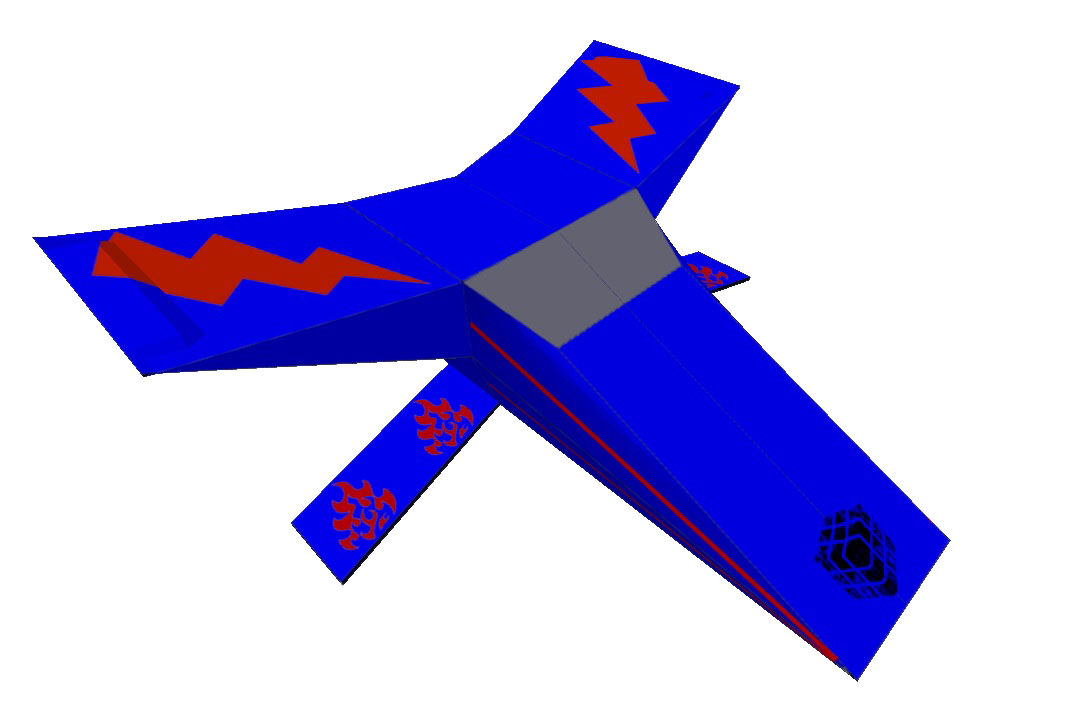
\includegraphics[height=6cm, width=9cm]{vaisseau_arthur.jpg}
\caption{L'un des vaisseaux fait par Arthur}

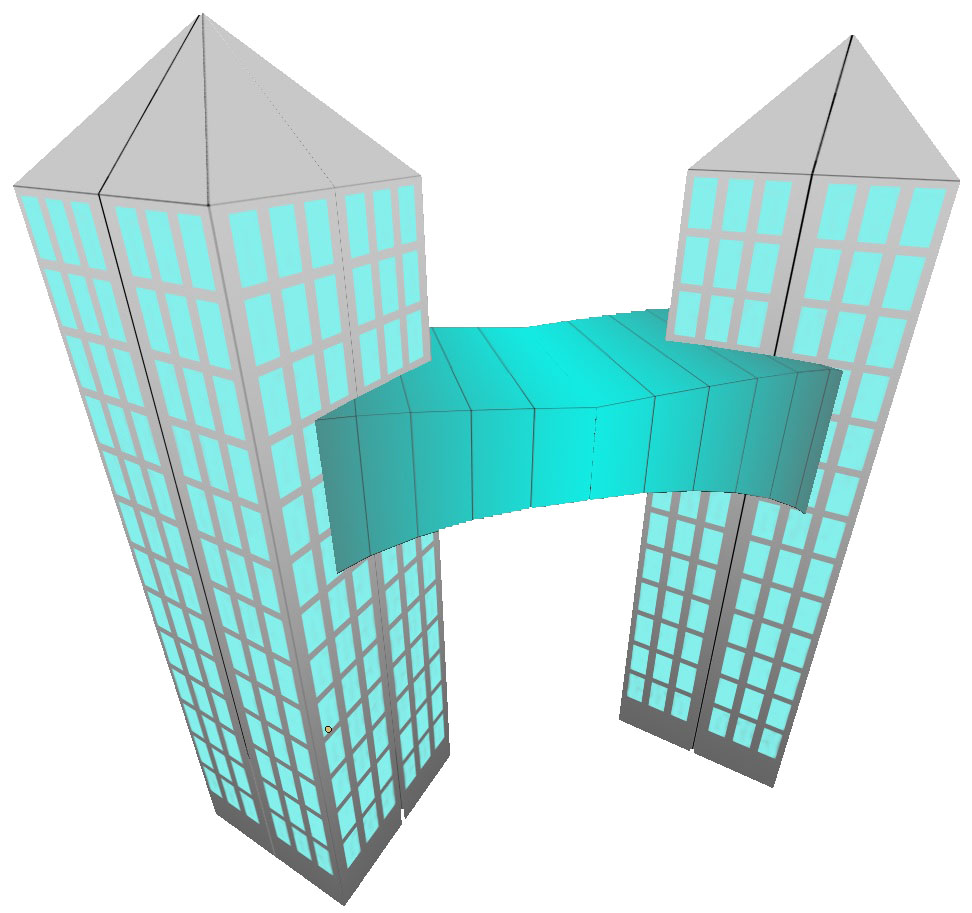
\includegraphics[height=8.5cm, width=8cm]{batiment_arthur.jpg}
\caption{L'un des immeubles fait par Arthur}

\end{figure}

\subsection{Ce qu'Arthur doit faire pour la prochaine soutenance}

Arthur continuera le script en C\# pour obtenir un meilleur gameplay. Il va principalement gérer la mort du joueur et la destruction de son vaisseau avec une animation et un écran qui affiche que l'on est mort et aussi une réaparition dans le niveau. 

 Il va aussi rechercher si on peut modifier la vue de la caméra pour qu'elle se mouve en fonction des rotations du vaisseau contrôlé par le joueur. Cela améliorerait le visuel du jeu et éviterait dans rendre malade le joueur à force de jouer.\\

Il va commencer l'I.A avec Guillaume pour que l'on puisse jouer avec ou contre l'ordinateur.

\chapter{Pour la prochaine soutenance}

Tout d'abord, nous allons améliorer le contenu : nous allons rajouter des vaisseaux, des niveaux, des bâtiments\dots etc.\\
Le menu sera complété, notamment dans les options et dans le choix de son vaisseau pour que le joueur puisse plus facilement personnaliser sa manière de jouer, avec peut-être aussi l'apparition de sauvegardes.
Le site web sera commencé en \bsc{html}, pour pouvoir tenir au courant tous les fans qui suivent notre projet et veulent télécharger les dernières versions de notre jeu.\\

Mais surtout, la prochaine soutenance verra l'apparition des \textbf{I.A}. Avec cela, le joueur pourra jouer contre des ennemis gérés par l'ordinateur qu'il devra détruire, tout en essayant de ne pas se faire exploser par eux !\\

 Et surtout, le \textbf{multijoueur en réseau local} sera commencé ! Il ne sera sans doute pas déjà opérationnel à 100\% pour la prochaine soutenance, .

\end{document}